% graphics source https://docs.google.com/presentation/d/111HE56Ow0miZApHPBa18eyPAw8cdslZyBCavoWMix8E
\begin{figure}[htb]
\centering
\begin{minipage}{0.47\linewidth}
\centering
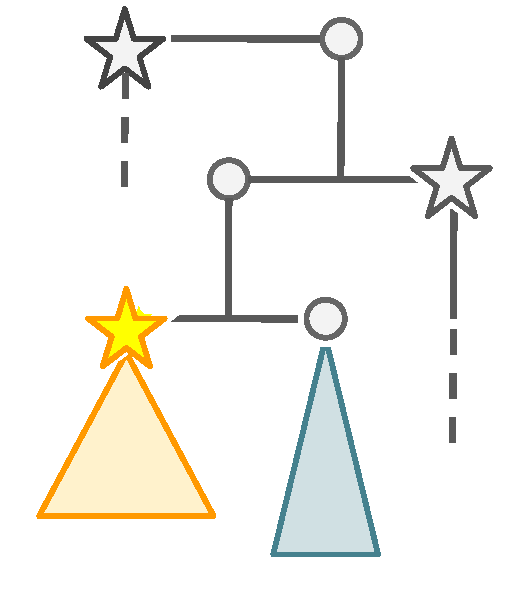
\includegraphics[width=0.7\linewidth]{img/screen-strategy-tree-balance}
\subcaption{one sister clade comparator}
\label{fig:screen-strategy:tree-balance}
\end{minipage}
~~
\begin{minipage}{0.47\linewidth}
\centering
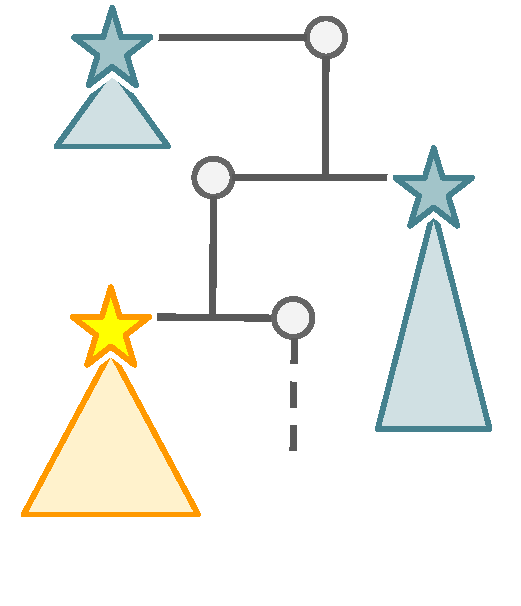
\includegraphics[width=0.7\linewidth]{img/screen-strategy-comparator}
\subcaption{multiple MDC comparators}
\label{fig:screen-strategy:window}
\end{minipage}
\vspace{-1ex}
\caption{%
\textbf{Fitness-effect screen strategies.}
\footnotesize
Yellow star indicates mutation of interest, yellow triangle indicates the clade it defines. Teal triangles indicate comparator clades. Teal stars indicate mutations defining comparator clades. Grey stars indicate mutations defining clades that are neither the focal clade nor comparator clades.
a) As proposed by \citep{BonettiFranceschi2024phylogenetic}, the focal clade is compared to its sister clade (which may or may not be mutation-defined), b) The focal clade is compared to a collection of other mutation-defined clades (MDCs).
}
\label{fig:screen-strategy}
\end{figure}
